\documentclass[utf8,compress,aspectratio=169]{beamer}
\usepackage{irbookslide}
\usepackage{irilmenau2}
\usepackage{url}
\usepackage{fontspec} % zahteva paket euenc
\usepackage{xunicode}
\usepackage{xltxtra}
\usepackage{polyglossia}
\usepackage{xcolor,colortbl}
\usepackage{textcomp}
\usepackage{unicode-math}

\usepackage[cache=false]{minted}
\AtBeginEnvironment{minted}{\dontdofcolorbox}
\def\dontdofcolorbox{\renewcommand\fcolorbox[4][]{##4}}

\usepackage{hyperref}
\hypersetup{pdfstartview=Fit}

\usepackage{tikz}
\usetikzlibrary{
  arrows,
  arrows.meta,
  shapes.geometric,
  shapes.multipart,
  quotes,
  positioning,
  tikzmark,
  chains
}

\title{Funkcije}
\subtitle{\tiny{Slajdovi za predmet Osnove programiranja}}
\subject{Osnove programiranja}
\institute{Katedra za informatiku, Fakultet tehničkih nauka, Novi Sad}
\date{2021.}

\begin{document}

% da pygmentize ne uokviruje crvenom bojom nepoznate karaktere
\expandafter\def\csname PY@tok@err\endcsname{}

\frame{\titlepage}

\frame{
  \frametitle{Ciljevi}
  \begin{itemize}
    \item razumevanje zašto je korisno podeliti program u skup više potprograma (funkcija)
    \item poznavanje pisanja funkcija u Pythonu
    \item poznavanje detalja pozivanja funkcija i prenosa parametara
    \item pisanje programa koji koriste funkcije -- radi povećanja modularnosti i izbegavanja ponavljanja koda
  \end{itemize}
}

\section{Pojam funkcije}

\frame{
  \frametitle{Funkcija funkcija}
  \begin{itemize}
    \item do sada smo videli različite vrste funkcija:
    \item u nekim primerima program se sastojao od jedne funkcije \texttt{main}
    \item ugrađene funkcije, npr. \texttt{abs}
    \item funkcije iz paketa, npr. \texttt{math.sqrt}
  \end{itemize}
}

\frame{
  \frametitle{Funkcija funkcija $_2$}
  \begin{itemize}
    \item imati isti programski kod na više mesta donosi probleme
    \item problem \myblue{1}: pisanje istog koda više puta je više posla
    \item problem \myblue{2}: isti kod se mora održavati na više mesta istovremeno
    \item funkcije se mogu upotrebiti protiv ponavljanja istog koda, i pomažu da programi budu čitljiviji i lakši za održavanje
  \end{itemize}
}

\frame{
  \frametitle{Funkcija funkcija $_3$}
  \begin{itemize}
    \item funkcija je kao potprogram, mali program unutar većeg programa
    \item osnovna ideja -- napišemo niz naredbi i dodelimo mu ime;
    \item kasnije izvršavamo taj niz naredbi pozivajući ga po imenu
  \end{itemize}
}

\frame{
  \frametitle{Funkcija funkcija $_4$}
  \begin{itemize}
    \item deo programa u kome se funkcija kreira zove se \myblue{definicija funkcije}
    \item kada se funkcija koristi u programu, kažemo da se ona \myblue{poziva}
  \end{itemize}
}

\begin{frame}[fragile]
  \frametitle{Primer funkcija}
  \begin{itemize}
    \item definicija funkcije
  \end{itemize}
\begin{minted}[linenos=false]{python}
def main():
    print("Happy birthday to you!")
    print("Happy birthday to you!")
    print("Happy birthday, dear Fred...")
    print("Happy birthday to you!")
\end{minted}
  \begin{itemize}
    \item poziv funkcije
  \end{itemize}
\begin{verbatim}
>>> main()
Happy birthday to you!
Happy birthday to you!
Happy birthday, dear Fred...
Happy birthday to you!
\end{verbatim}
\end{frame}

\begin{frame}[fragile]
  \frametitle{Primer funkcija $_2$}
  \begin{itemize}
    \item imamo ponavljanje u kodu: \\
      \texttt{print("Happy birthday to you!")}
    \item možemo napisati funkciju koja ispisuje ovaj red:
  \end{itemize}
\begin{minted}[linenos=false]{python}
def happy():
    print("Happy birthday to you!")
\end{minted}
  \begin{itemize}
    \item sada možemo da skratimo naš program
  \end{itemize}
\end{frame}

\begin{frame}[fragile]
  \frametitle{Primer funkcija $_3$}
  \begin{itemize}
    \item novi program
  \end{itemize}
\begin{minted}[linenos=false]{python}
def singFred():
    happy()
    happy()
    print("Happy birthday, dear Fred...")
    happy()
\end{minted}
  \begin{itemize}
    \item rezultat je:
  \end{itemize}
\begin{verbatim}
>>> singFred()
Happy birthday to you!
Happy birthday to you!
Happy birthday, dear Fred...
Happy birthday to you!
\end{verbatim}
\end{frame}

\begin{frame}[fragile]
  \frametitle{Primer funkcija $_4$}
  \begin{itemize}
    \item funkcija \texttt{happy} nam je uštedela dosta kucanja
    \item šta ako nam treba rođendan za Lucy?
    \item mogli bismo napisati funkciju za Lucy:
  \end{itemize}
\begin{minted}[linenos=false]{python}
def singLucy():
    happy()
    happy()
    print("Happy birthday, dear Lucy...")
    happy()
\end{minted}
\end{frame}

\begin{frame}[fragile,shrink=10]
  \frametitle{Primer funkcija $_5$}
  \begin{itemize}
    \item možemo napisati program za Freda i Lucy
  \end{itemize}
\begin{minted}[linenos=false]{python}
def main():
    singFred()
    print()
    singLucy()
\end{minted}
  \begin{itemize}
    \item dobićemo ovaj rezultat
  \end{itemize}
\begin{verbatim}
>>> main()
Happy birthday to you!
Happy birthday to you!
Happy birthday, dear Fred..
Happy birthday to you!

Happy birthday to you!
Happy birthday to you!
Happy birthday, dear Lucy...
Happy birthday to you!
\end{verbatim}
\end{frame}

\begin{frame}[fragile]
  \frametitle{Primer funkcija $_5$}
  \begin{itemize}
    \item još uvek ima ponavljanja koda
    \item jedina razlika između \texttt{singFred} i \texttt{singLucy} je ime u trećoj naredbi
    \item od ove dve funkcije može se napraviti jedna, sa parametrom
  \end{itemize}
\end{frame}

\begin{frame}[fragile]
  \frametitle{Primer funkcija $_6$}
  \begin{itemize}
    \item opštija funkcija \texttt{sing}
  \end{itemize}
\begin{minted}[linenos=false]{python}
def sing(person):
    happy()
    happy()
    print("Happy birthday, dear", person + ".")
    happy()
\end{minted}
  \begin{itemize}
    \item ova funkcija ima \myblue{parametar} sa nazivom \texttt{person}
    \item parametar je promenljiva čija vrednost se definiše prilikom poziva funkcije
  \end{itemize}
\end{frame}

\begin{frame}[fragile]
  \frametitle{Primer funkcija $_7$}
  \begin{itemize}
    \item novi izlaz iz programa je:
  \end{itemize}
\begin{verbatim}
>>> sing("Fred")
Happy birthday to you!
Happy birthday to you!
Happy birthday, dear Fred.
Happy birthday to you!
\end{verbatim}
  \begin{itemize}
    \item sada možemo da preradimo i glavni program
  \end{itemize}
\end{frame}

\begin{frame}[fragile,shrink=10]
  \frametitle{Primer funkcija $_8$}
  \begin{itemize}
    \item novi glavni program glasi:
  \end{itemize}
\begin{minted}[linenos=false]{python}
def main():
    sing("Fred")
    print()
    sing("Lucy")
\end{minted}
  \begin{itemize}
    \item rezultat je sada sledeći:
  \end{itemize}
\begin{verbatim}
>>> main()
Happy birthday to you!
Happy birthday to you!
Happy birthday, dear Fred.
Happy birthday to you!

Happy birthday to you!
Happy birthday to you!
Happy birthday, dear Lucy.
Happy birthday to you!
\end{verbatim}
\end{frame}

\section{Parametri}

\begin{frame}[fragile]
  \frametitle{Funkcije i parametri}
  \begin{itemize}
    \item \myblue{opseg} (scope) promenljive definiše deo programa u kome se promenljiva može koristiti
    \item svaka funkcija je poseban potprogram
    \item promenljive koje se koriste unutar funkcije su \myblue{lokalne} za tu funkciju
    \item makar imale isto ime kao i neke promenljive izvan te funkcije \\ \ \\
    \item jedini način da funkcija ,,vidi`` podatak izvan sebe je da ga dobije kao parametar
  \end{itemize}
\end{frame}

\begin{frame}[fragile]
  \frametitle{Funkcije i parametri $_2$}
  \begin{itemize}
    \item definicija funkcije izgleda ovako: \\
      \texttt{def <name>(<formal-parameters>):} \\
      \texttt{\ \ \ \ <body>}
    \item ime funkcije (\texttt{name}) mora biti identifikator
    \item \texttt{formal-parameters} je lista imena parametara (lista može biti prazna)
  \end{itemize}
\end{frame}

\begin{frame}[fragile]
  \frametitle{Funkcije i parametri $_3$}
  \begin{itemize}
    \item formalni parametri su dostupni samo u telu funkcije
    \item promenljive sa istim imenom u drugim delovima programa su različite od parametara i lokalnih promenljivih u funkciji
  \end{itemize}
\end{frame}

\begin{frame}[fragile]
  \frametitle{Funkcije i parametri $_4$}
  \begin{itemize}
    \item funkcija se poziva po imenu za kojim sledi lista \myblue{stvarnih parametara} ili \myblue{argumenata}: \\
      \texttt{<name>(<actual-parameters>)}
  \end{itemize}
\end{frame}

\begin{frame}[fragile]
  \frametitle{Poziv funkcije}
  \begin{itemize}
    \item kada Python naiđe na poziv funkcije, otpočinje proces od 4 koraka:
    \item[1] pozivajući program zaustavlja izvršavanje u tački poziva funkcije
    \item[2] formalni parametri funkcije dobijaju vrednosti stvarnih parametara iz poziva
    \item[3] telo funkcije se izvršava
    \item[4] kontrola se vraća u tačku odmah iza poziva funkcije
  \end{itemize}
\end{frame}

\begin{frame}[fragile]
  \frametitle{Poziv funkcije $_2$}
  \begin{itemize}
    \item prođimo kroz sledeći kod:
  \end{itemize}
\begin{minted}[linenos=false]{python}
sing("Fred")
print()
sing("Lucy")
\end{minted}
  \begin{itemize}
    \item kada Python naiđe na \texttt{sing("Fred")}, izvršavanje \texttt{main} se privremeno zaustavlja
    \item Python traži definiciju funkcije \texttt{sing} i vidi da ona ima jedan formalni parametar, \texttt{person}
  \end{itemize}
\end{frame}

\begin{frame}[fragile]
  \frametitle{Poziv funkcije $_3$}
  \begin{itemize}
    \item formalni parametar dobija vrednost stvarnog parametra
    \item to je kao da smo izvršili sledeću naredbu
  \end{itemize}
\begin{minted}[linenos=false]{python}
person = "Fred"
\end{minted}
  \begin{itemize}
    \item promenljiva \texttt{person} je upravo inicijalizovana
  \end{itemize}
\begin{minted}[escapeinside=??,linenos=false,fontsize=\footnotesize]{python}
                                def sing(person):
def main():                         ?\tikzmark{end1}?happy()
    sing("Fred")?\tikzmark{start1}?                    happy()
    print()                         print("Happy birthday, dear",
    sing("Lucy")                          person + ".")
                                    happy()
\end{minted}
\begin{tikzpicture}[remember picture]
\draw[overlay,->,red,line width=2pt,sloped] (pic cs:start1) -- (pic cs:end1) node[midway,above] {\footnotesize{\texttt{person="Fred"}}};
\end{tikzpicture}
\end{frame}

\begin{frame}[fragile]
  \frametitle{Poziv funkcije $_4$}
  \begin{itemize}
    \item u ovom trenutku Python počinje izvršavanje tela funkcije \texttt{sing}
    \item prva naredba je poziv funkcije \texttt{happy}
    \item Python zaustavlja izvršavanje funkcije \texttt{sing} i prebacuje kontrolu na \texttt{happy}
    \item funkcija \texttt{happy} se sastoji iz jedne \texttt{print} naredbe koja se izvrši i kontrola se vraća nazad
  \end{itemize}
\end{frame}

\begin{frame}[fragile]
  \frametitle{Poziv funkcije $_5$}
\begin{minted}[escapeinside=??,linenos=false,fontsize=\scriptsize]{python}
def main():             def sing(person):           def happy():
    sing("Fred")?\tikzmark{start2}?            ?\tikzmark{end2}?happy()?\tikzmark{start3}?                     ?\tikzmark{end3}?print("Happy birthday to you!")
    print()                 happy()                     ?\tikzmark{start4}?
    sing("Lucy")            print("dear", person)
                            happy()
\end{minted}
\begin{tikzpicture}[remember picture]
  \draw[overlay,->,red,line width=1pt,sloped] (pic cs:start2) -- ([xshift=-5]pic cs:end2) node[midway,above] {\tiny{\texttt{person="Fred"}}};
  \draw[overlay,->,red,line width=1pt,sloped] (pic cs:start3) -- ([xshift=-5]pic cs:end3);
  \draw[overlay,->,red,line width=1pt,sloped] ([xshift=-5]pic cs:end3) -- ([xshift=-5]pic cs:start4);
  \draw[overlay,->,red,line width=1pt,sloped] ([xshift=-5]pic cs:start4) -- (pic cs:start3);
\end{tikzpicture}
\begin{itemize}
  \item izvršavanje se nastavlja sa još dva poziva funkcije \texttt{happy}
  \item kada Python dođe do kraja funkcije \texttt{sing}, vraća kontrolu nazad funkciji \texttt{main}
  \item tamo nastavlja izvršavanje odmah posle poziva funkcije \texttt{sing}
\end{itemize}
\end{frame}

\begin{frame}[fragile]
  \frametitle{Poziv funkcije $_6$}
\begin{minted}[escapeinside=??,linenos=false,fontsize=\footnotesize]{python}
                            def sing(person):
def main():                         ?\tikzmark{end5}?happy()
    sing("Fred")?\tikzmark{start5}?                    happy()
    print()                         print("Happy birthday, dear",
    sing("Lucy")                          person + ".")
                                    ?\tikzmark{start6}?happy()
\end{minted}
\begin{tikzpicture}[remember picture]
  \draw[overlay,->,red,line width=1pt,sloped] (pic cs:start5) -- ([xshift=-5]pic cs:end5) node[midway,above] {\footnotesize{\texttt{person="Fred"}}};
  \draw[overlay,->,red,line width=1pt] ([xshift=-5]pic cs:end5) -- ([xshift=-5]pic cs:start6);
  \draw[overlay,->,red,line width=1pt] ([xshift=-5]pic cs:start6) -- (pic cs:start5);
\end{tikzpicture}
\begin{itemize}
    \item promenljiva \texttt{person} u funkciji \texttt{main} nije vidljiva!
    \item memorija koju zauzimaju lokalne promenljive dok se funkcija izvršava se oslobađa nakon završetka funkcije
    \item lokalne promenljive ne čuvaju vrednost između dva poziva funkcije
  \end{itemize}
\end{frame}

\begin{frame}[fragile]
  \frametitle{Poziv funkcije $_7$}
  \begin{itemize}
    \item sledeća naredba je \texttt{print()} koja ispisuje prazan red
    \item Python nailazi na još jedan poziv funkcije \texttt{sing}
    \item prenosi kontrolu na funkciju \texttt{sing}, a parametar ima vrednost \texttt{"Lucy"}
  \end{itemize}
\begin{minted}[escapeinside=??,linenos=false,fontsize=\footnotesize]{python}
                            def sing(person):
def main():                         ?\tikzmark{pin04}?happy()
    ?\tikzmark{pin01}?sing("Fred")                    happy()
    print()                         print("Happy birthday, dear",
    ?\tikzmark{pin02}?sing("Lucy")?\tikzmark{pin03}?                          person + ".")
                                    happy()
\end{minted}
\begin{tikzpicture}[remember picture]
  \draw[overlay,->,red,line width=1pt,sloped] (pic cs:pin03) -- (pic cs:pin04) node[midway,above] {\footnotesize{\texttt{person="Lucy"}}};
  \draw[overlay,->,red,line width=1pt] ([xshift=-5]pic cs:pin01) -- ([xshift=-5]pic cs:pin02);
\end{tikzpicture}
\end{frame}

\begin{frame}[fragile]
  \frametitle{Poziv funkcije $_8$}
  \begin{itemize}
    \item telo funkcije \texttt{sing} sada se izvršava sa parametrom \texttt{"Lucy"}
    \item to uključuje tri poziva funkcije \texttt{happy}
    \item na kraju se kontrola prenosi nazad u \texttt{main}
  \end{itemize}
\begin{minted}[escapeinside=??,linenos=false,fontsize=\footnotesize]{python}
                            def sing(person):
def main():                         ?\tikzmark{pin08}?happy()
    ?\tikzmark{pin05}?sing("Fred")                    happy()
    print()                         print("Happy birthday, dear",
    ?\tikzmark{pin06}?sing("Lucy")?\tikzmark{pin07}?                          person + ".")
                                    ?\tikzmark{pin09}?happy()
\end{minted}
\begin{tikzpicture}[remember picture]
  \draw[overlay,->,red,line width=1pt] ([xshift=-5]pic cs:pin05) -- ([xshift=-5]pic cs:pin06);
  \draw[overlay,->,red,line width=1pt] (pic cs:pin07) -- ([xshift=-5]pic cs:pin08);
  \draw[overlay,->,red,line width=1pt] ([xshift=-5]pic cs:pin08) -- ([xshift=-5]pic cs:pin09);
  \draw[overlay,->,red,line width=1pt] ([xshift=-5]pic cs:pin09) -- ([xshift=5]pic cs:pin07);
  \draw[overlay,->,red,line width=1pt] ([xshift=-5,yshift=-5]pic cs:pin06) -- ([xshift=-5,yshift=-15]pic cs:pin06);
\end{tikzpicture}
\end{frame}

\begin{frame}[fragile]
  \frametitle{Poziv funkcije $_9$}
  \begin{itemize}
    \item prosleđivanje parametara je mehanizam za inicijalizaciju promenljivih u funkciji
    \item parametri predstavljaju \myblue{ulazne} podatke za funkciju
    \item možemo pozivati funkciju više puta sa različitim parametrima i dobiti različite rezultate
  \end{itemize}
\end{frame}

\section{Rezultat}

\begin{frame}[fragile]
  \frametitle{Rezultat funkcije}
  \begin{itemize}
    \item videli smo primere funkcija koje vraćaju vrednost onome ko ih poziva \\
      \texttt{root = math.sqrt(b*b - 4*a*c)}
    \item vrednost \texttt{b*b - 4*a*c} je stvarni parametar poziva funkcije \texttt{math.sqrt}
    \item kažemo da \texttt{math.sqrt} \myblue{vraća} kvadratni koren svog argumenta
  \end{itemize}
\end{frame}

\begin{frame}[fragile]
  \frametitle{Rezultat funkcije $_2$}
  \begin{itemize}
    \item ova funkcija vraća kvadrat datog broja: \\
  \end{itemize}
\begin{minted}[linenos=false]{python}
def square(x):
    return x*x
\end{minted}
  \begin{itemize}
    \item kada Python naiđe na \texttt{return} vraća se nazad iz funkcije i predaje kontrolu u tački gde je funkcija pozvana
    \item vrednost data u \texttt{return} naredbi se šalje nazad onome ko je pozvao funkciju
  \end{itemize}
\end{frame}

\begin{frame}[fragile]
  \frametitle{Rezultat funkcije $_3$}
\begin{minted}[linenos=false]{python}
>>> square(3)
9
>>> print(square(4))
16
>>> x = 5
>>> y = square(x)
>>> print(y)
25
>>> print(square(x) + square(3))
34
\end{minted}
\end{frame}

\begin{frame}[fragile]
  \frametitle{Rezultat funkcije $_4$}
  \begin{itemize}
    \item možemo da iskoristimo funkciju \texttt{square} da napravimo funkciju za rastojanje dve tačke $(x_1,y_1)$ i $(x_2,y_2)$
  \end{itemize}
\begin{minted}[linenos=false]{python}
def distance(x1, y1, x2, y2):
    dist = math.sqrt(square(x2 - x1) + square(y2 - y1))
    return dist
\end{minted}
\end{frame}

\begin{frame}[fragile]
  \frametitle{Rezultat funkcije $_5$}
  \begin{itemize}
    \item nekad funkcija mora da vrati više od jedne vrednosti
    \item rezultat funkcije može biti lista ili sekvenca vrednosti
  \end{itemize}
\begin{minted}[linenos=false]{python}
def sumDiff(x, y):
    sum = x + y
    diff = x - y
    return sum, diff
\end{minted}
\end{frame}

\begin{frame}[fragile,shrink=5]
  \frametitle{Rezultat funkcije $_6$}
  \begin{itemize}
    \item kada se poziva ovakva funkcija, koristi se istovremena dodela više vrednosti
  \end{itemize}
\begin{minted}[linenos=false]{python}
n1, n2 = eval(input("Unesite dva broja (n1, n2): "))
s, d = sumDiff(n1, n2)
print("Zbir je", s, "a razlika je", d)
\end{minted}
  \begin{itemize}
    \item vrednosti se dodeljuju prema poziciji
    \item \texttt{s} će dobiti prvu vrednost, a \texttt{d} drugu
  \end{itemize}
\end{frame}

\begin{frame}[fragile]
  \frametitle{Rezultat funkcije $_7$}
  \begin{itemize}
    \item sitna fora: sve Python funkcije vraćaju vrednost
    \item bez obzira da li postoji \texttt{return} ili ne
    \item ako ne postoji \texttt{return} vraća se specijalna vrednost \texttt{None}
    \item \texttt{return} se često zaboravi u pisanju koda!
    \begin{itemize}
      \item ako se prilikom poziva funkcije dobijaju čudne greške, prvo proveriti ovo
    \end{itemize}
  \end{itemize}
\end{frame}

\section{Prenos parametara}

\begin{frame}[fragile]
  \frametitle{Izmena parametara}
  \begin{itemize}
    \item rezultat funkcije je osnovni način da se informacije vrate nazad onome ko poziva funkciju
    \item rezultat rada funkcije se može preneti nazad i tako što se parametar funkcije promeni
    \item razumevanje ovog postupka traži dublje poznavanje mehanizma dodele vrednosti i prenosa parametara
  \end{itemize}
\end{frame}

\begin{frame}[fragile]
  \frametitle{Izmena parametara $_2$}
  \begin{itemize}
    \item recimo da pišemo program koji upravlja bankovnim računima
    \item treba nam funkcija koja dodaje kamatu na račun
    \item prva verzija funkcije
  \end{itemize}
\begin{minted}[linenos=false]{python}
def addInterest(balance, rate):
    newBalance = balance * (1 + rate)
    balance = newBalance
\end{minted}
\end{frame}

\begin{frame}[fragile]
  \frametitle{Izmena parametara $_3$}
  \begin{itemize}
    \item ideja je da se pomeni \texttt{balance} tako da se poveća za iznos kamate
    \item napišimo program za test:
  \end{itemize}
\begin{minted}[linenos=false]{python}
def test():
    amount = 1000
    rate = 0.05
    addInterest(amount, rate)
    print(amount)
\end{minted}
\end{frame}

\begin{frame}[fragile]
  \frametitle{Izmena parametara $_4$}
  \begin{itemize}
    \item nadamo se da će 5\% biti dodato na račun i da će rezultat biti 1050
  \end{itemize}
\begin{minted}[linenos=false]{python}
>>> test()
1000
\end{minted}
  \begin{itemize}
    \item nema greške, sve je u redu!
  \end{itemize}
\end{frame}

\begin{frame}[fragile,shrink=10]
  \frametitle{Izmena parametara $_5$}
\begin{tabular}{p{4cm}p{8cm}}
  \begin{itemize}
    \item[1] prve dve linije u \texttt{test}-u kreiraju dve lokalne promenljive, \texttt{amount} i \texttt{rate}
    \item[2] one dobijaju vrednosti 1000 i 0.05
  \end{itemize}
&
\begin{minted}[linenos=false]{python}
def addInterest(balance, rate):
    newBalance = balance * (1 + rate)
    balance = newBalance

def test():
    amount = 1000
    rate = 0.05
    addInterest(amount, rate)
    print(amount)
\end{minted}
\end{tabular}
\end{frame}

\begin{frame}[fragile,shrink=10]
  \frametitle{Izmena parametara $_5$}
\begin{tabular}{p{4cm}p{8cm}}
  \begin{itemize}
    \item[3] kontrola se dalje prenosi na funkciju \texttt{addInterest}
    \item[4] formalni parametri \texttt{balance} i \texttt{rate} dobijaju vrednosti stvarnih parametara \texttt{amount} i \texttt{rate}
    \item[5] iako \texttt{rate} postoji u obe funkcije, to su dve različite promenljive
  \end{itemize}
&
\begin{minted}[linenos=false]{python}
def addInterest(balance, rate):
    newBalance = balance * (1 + rate)
    balance = newBalance

def test():
    amount = 1000
    rate = 0.05
    addInterest(amount, rate)
    print(amount)
\end{minted}
\end{tabular}
\end{frame}

\begin{frame}[fragile,shrink=10]
  \frametitle{Izmena parametara $_6$}
\begin{tabular}{p{4cm}p{8cm}}
  \begin{itemize}
    \item[6] dodela vrednosti za parametre \texttt{balance} i \texttt{rate} funkcije \texttt{addInterest} koristi vrednosti \myblue{stvarnih} parametara
  \end{itemize}
&
\begin{minted}[linenos=false]{python}
def addInterest(balance, rate):
    newBalance = balance * (1 + rate)
    balance = newBalance

def test():
    amount = 1000
    rate = 0.05
    addInterest(amount, rate)
    print(amount)
\end{minted}
\end{tabular}
\end{frame}

\begin{frame}[fragile,shrink=10]
  \frametitle{Izmena parametara $_7$}

\begin{minted}[escapeinside=??,linenos=false,fontsize=\footnotesize]{python}
def test():                                   ?\tikzmark{pin94}?def addInterest(balance, rate):
    ?\tikzmark{pin91}?amount = 1000                                 newBalance = balance * (1 + rate)
    rate = 0.05                                   balance = newBalance
    ?\tikzmark{pin92}?addInterest(amount, rate)?\tikzmark{pin93}?
    print(amount)
\end{minted}
\begin{tikzpicture}[remember picture]
  \draw[overlay,->,red,line width=1pt] ([xshift=-5]pic cs:pin91) -- ([xshift=-5]pic cs:pin92);
  \draw[overlay,->,red,line width=1pt] (pic cs:pin93) -- ([xshift=-5]pic cs:pin94) node[midway,above,text width=3cm,align=center] {\footnotesize{\texttt{balance=amount rate=rate}}};
\end{tikzpicture}

\ %

\begin{tikzpicture}[scale=1,transform shape,every text node part/.style={align=left}]
  \node[rectangle,draw=white,fill=white] (0) at (0,1) {amount};
  \node[rectangle,draw=black,fill=white] (5) at (2,1) {$1000$};
  \draw[->] (0) -- (5);
  \node[rectangle,draw=white,fill=white] (8) at (0,0) {rate};
  \node[rectangle,draw=black,fill=white] (9) at (2,0) {$0.05$};
  \draw[->] (8) -- (9);
  \node[rectangle,draw=white,fill=white] (1) at (8,1) {balance};
  \node[rectangle,draw=white,fill=white] (7) at (8,0) {rate};
  \draw[->] (1) -- (5);
  \draw[->] (7) -- (9);
\end{tikzpicture}

% \begin{center}
%   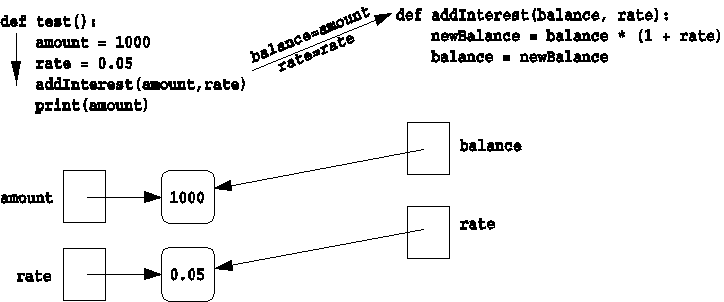
\includegraphics[width=14cm]{pic09}
% \end{center}
\end{frame}

\begin{frame}[fragile,shrink=10]
  \frametitle{Izmena parametara $_8$}
\begin{tabular}{p{4cm}p{8cm}}
  \begin{itemize}
    \item[7] izvršavanje prve linije u \texttt{addInterest} će kreirati novu promenljivu \texttt{newBalance}
    \item[8] u drugoj liniji će \texttt{balance} primiti vrednost od \texttt{newBalance}
  \end{itemize}
&
\begin{minted}[linenos=false]{python}
def addInterest(balance, rate):
    newBalance = balance * (1 + rate)
    balance = newBalance

def test():
    amount = 1000
    rate = 0.05
    addInterest(amount, rate)
    print(amount)
\end{minted}
\end{tabular}
\end{frame}

\begin{frame}[fragile,shrink=10]
  \frametitle{Izmena parametara $_9$}
\begin{tabular}{p{4cm}p{8cm}}
  \begin{itemize}
    \item[9] \texttt{balance} sada pokazuje na istu vrednost kao i \texttt{newBalance}
    \item[10] ali to nema uticaja na \texttt{amount} u \texttt{test}-u
  \end{itemize}
&
\begin{minted}[linenos=false]{python}
def addInterest(balance, rate):
    newBalance = balance * (1 + rate)
    balance = newBalance

def test():
    amount = 1000
    rate = 0.05
    addInterest(amount, rate)
    print(amount)
\end{minted}
\end{tabular}
\end{frame}

\begin{frame}[fragile,shrink=10]
  \frametitle{Izmena parametara $_{10}$}
\begin{minted}[escapeinside=??,linenos=false,fontsize=\footnotesize]{python}
def test():                                   ?\tikzmark{pin04}?def addInterest(balance, rate):
    ?\tikzmark{pin01}?amount = 1000                                 newBalance = balance * (1 + rate)
    rate = 0.05                                   balance = newBalance
    ?\tikzmark{pin02}?addInterest(amount, rate)?\tikzmark{pin03}?
    print(amount)
\end{minted}
\begin{tikzpicture}[remember picture]
  \draw[overlay,->,red,line width=1pt] ([xshift=-5]pic cs:pin01) -- ([xshift=-5]pic cs:pin02);
  \draw[overlay,->,red,line width=1pt] (pic cs:pin03) -- ([xshift=-5]pic cs:pin04) node[midway,above,text width=3cm,align=center] {\footnotesize{\texttt{balance=amount rate=rate}}};
\end{tikzpicture}

\ %

\begin{tikzpicture}[scale=1,transform shape,every text node part/.style={align=left}]
  \node[rectangle,draw=white,fill=white] (0) at (0,1) {amount};
  \node[rectangle,draw=black,fill=white] (5) at (2,1) {$1000$};
  \draw[->] (0) -- (5);
  \node[rectangle,draw=white,fill=white] (8) at (0,0) {rate};
  \node[rectangle,draw=black,fill=white] (9) at (2,0) {$0.05$};
  \draw[->] (8) -- (9);
  \node[rectangle,draw=black,fill=white] (6) at (5,-1) {$1050$};
  \node[rectangle,draw=white,fill=white] (1) at (8,1) {balance};
  \node[rectangle,draw=white,fill=white] (7) at (8,0) {rate};
  \node[rectangle,draw=white,fill=white] (4) at (8,-1) {newBalance};
  \draw[->] (1) -- (6);
  \draw[->] (4) -- (6);
  \draw[->] (7) -- (9);
\end{tikzpicture}

% \begin{center}
%   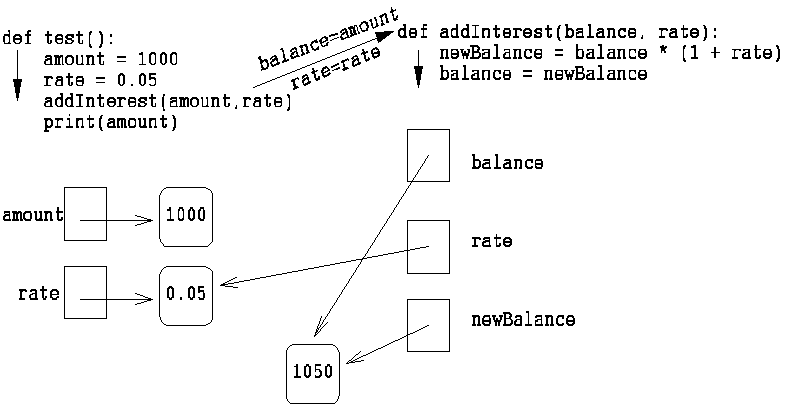
\includegraphics[width=14cm]{pic10}
% \end{center}
\end{frame}

\begin{frame}[fragile,shrink=10]
  \frametitle{Izmena parametara $_{11}$}
\begin{tabular}{p{4cm}p{8cm}}
  \begin{itemize}
    \item[10] izvršavanje \texttt{addInterest} se završava i kontrola se vraća \texttt{test}-u
    \item[11] lokalne promenljive iz \texttt{addInterest} više ne postoje, ali \texttt{amount} i \texttt{rate} u \texttt{test}-u pokazuju i dalje na stare vrednosti
  \end{itemize}
&
\begin{minted}[linenos=false]{python}
def addInterest(balance, rate):
    newBalance = balance * (1 + rate)
    balance = newBalance

def test():
    amount = 1000
    rate = 0.05
    addInterest(amount, rate)
    print(amount)
\end{minted}
\end{tabular}
\end{frame}

\begin{frame}[fragile]
  \frametitle{Izmena parametara $_{12}$}
  \begin{itemize}
    \item rezime: formalni parametri funkcije primaju samo \myblue{vrednosti} stvarnih parametara
    \item funkcija nema pristup promenljivoj koja čuva stvarni parametar \\ \ \\
    \item kaže se da Python sve parametre \myblue{prenosi po vrednosti}
    \item ,,pass by value``
  \end{itemize}
\end{frame}

\begin{frame}[fragile]
  \frametitle{Izmena parametara $_{13}$}
  \begin{itemize}
    \item neki drugi jezici (C++, itd) omogućavaju da se se same promenljive (a ne njihove vrednosti) prenesu kao parametar poziva funkcije
    \item ovaj mehanizam se zove \myblue{prenos po referenci}
    \item ,,pass by reference``
    \item tada se izmene parametara unutar funkcije vide nakon njenog poziva
  \end{itemize}
\end{frame}

\begin{frame}[fragile]
  \frametitle{Izmena parametara $_{14}$}
  \begin{itemize}
    \item Python nema ovu mogućnost
    \item možemo izmeniti \texttt{addInterest} tako da vraća \texttt{newBalance}
  \end{itemize}
\begin{minted}[linenos=false]{python}
def addInterest(balance, rate):
    newBalance = balance * (1 + rate)
    return newBalance

def test():
    amount = 1000
    rate = 0.05
    amount = addInterest(amount, rate)
    print(amount)
\end{minted}
\end{frame}

\begin{frame}[fragile]
  \frametitle{Izmena parametara $_{15}$}
  \begin{itemize}
    \item umesto da radimo sa jednim bankovnim računom, možemo da radimo sa više računa
    \item račune možemo čuvati u listi
    \item i kamatu dodavati na svaki račun u listi
    \item prvi račun bi se mogao menjati ovako:
  \end{itemize}
\begin{minted}[linenos=false]{python}
balances[0] = balances[0] * (1 + rate)
\end{minted}
\end{frame}

\begin{frame}[fragile]
  \frametitle{Izmena parametara $_{16}$}
\begin{minted}[linenos=false]{python}
balances[0] = balances[0] * (1 + rate)
\end{minted}
  \begin{itemize}
    \item ovo znači ,,pomnoži vrednost nultog elementa liste sa \texttt{1+rate} i to smesti nazad u nulti element liste``
    \item opštiji način da ovo uradimo bio bi pomoću petlje koja ide kroz listu sa indeksom 0, 1, ..., dužina-1
  \end{itemize}
\end{frame}

\begin{frame}[fragile]
  \frametitle{Izmena parametara $_{17}$}
\begin{minted}[linenos=false]{python}
def addInterest(balances, rate):
    for i in range(len(balances)):
        balances[i] = balances[i] * (1+rate)

def test():
    amounts = [1000, 2200, 800, 360]
    rate = 0.05
    addInterest(amounts, 0.05)
    print(amounts)
\end{minted}
\end{frame}

\begin{frame}[fragile]
  \frametitle{Izmena parametara $_{18}$}
  \begin{itemize}
    \item početne vrednosti računa su bile \\
      \texttt{[1000, 2200, 800, 360]}
    \item program je vratio \\
      \texttt{[1050.0, 2310.0, 840.0, 378.0]}
    \item šta se desilo? izgleda kao da je \texttt{amounts} promenjen?
  \end{itemize}
\end{frame}

\begin{frame}[fragile,shrink=10]
  \frametitle{Izmena parametara $_{19}$}
\begin{tabular}{p{4cm}p{8cm}}
  \begin{itemize}
    \item[1] prve dve linije u \texttt{test}-u inicijalizuju promenljive \texttt{amounts} i \texttt{rate}
    \item[2] vrednost promenljive \texttt{amounts} je lista koja sadrži 4 int vrednosti
  \end{itemize}
&
\begin{minted}[linenos=false]{python}
def addInterest(balances, rate):
    for i in range(len(balances)):
        balances[i] = balances[i] *
            (1+rate)

def test():
    amounts = [1000, 2200, 800, 360]
    rate = 0.05
    addInterest(amounts, 0.05)
    print(amounts)
\end{minted}
\end{tabular}
\end{frame}

\begin{frame}[fragile]
  \frametitle{Izmena parametara $_{20}$}
\begin{minted}[escapeinside=??,linenos=false,fontsize=\footnotesize]{python}
def test():                                   def addInterest(balance, rate):
    ?\tikzmark{pin81}?amounts = [1000, 2150, 800, 3275]             for i in range(len(balances)):
    rate = 0.05                                       balances[i] = balances[i]*(1+rate)
    ?\tikzmark{pin82}?addInterest(amounts, rate)
    ?\tikzmark{pin83}?print(amounts)
\end{minted}
\begin{tikzpicture}[remember picture]
  \draw[overlay,->,red,line width=1pt] ([xshift=-5]pic cs:pin81) -- ([xshift=-5]pic cs:pin82);
  %\draw[overlay,->,red,line width=1pt] ([xshift=-5]pic cs:pin82) -- ([xshift=-5]pic cs:pin83);
\end{tikzpicture}

\ %

\begin{tikzpicture}[scale=1,transform shape,every text node part/.style={align=left}]
  \node[rectangle,draw=white,fill=white] (0) at (0,0) {amounts};
  \begin{scope}[start chain=1 going right,node distance=0cm]
    \node[rectangle,draw=black,fill=white,on chain=1] (1) at (2,0) {$\cdot$};
    \node[rectangle,draw=black,fill=white,on chain=1] (2) {$\cdot$};
    \node[rectangle,draw=black,fill=white,on chain=1] (3) {$\cdot$};
    \node[rectangle,draw=black,fill=white,on chain=1] (4) {$\cdot$};
  \end{scope}
  \draw[->] (0) -- (1);
  \node[rectangle,draw=black,fill=white] (5) at (1, -1) {$1000$};
  \node[rectangle,draw=black,fill=white] (6) at (3, -1) {$2150$};
  \node[rectangle,draw=black,fill=white] (7) at (5, -1) {$800$};
  \node[rectangle,draw=black,fill=white] (10) at (7, -1) {$3275$};
  \draw[->] (1) -- (5);
  \draw[->] (2) -- (6);
  \draw[->] (3) -- (7);
  \draw[->] (4) -- (10);

  \node[rectangle,draw=white,fill=white] (8) at (0,1) {rate};
  \node[rectangle,draw=black,fill=white] (9) at (2,1) {$0.05$};
  \draw[->] (8) -- (9);
\end{tikzpicture}

% \begin{center}
%   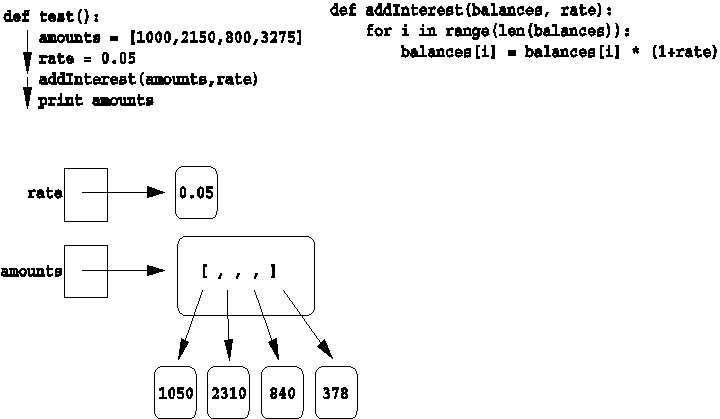
\includegraphics[width=12cm]{pic11}
% \end{center}
\end{frame}

\begin{frame}[fragile,shrink=10]
  \frametitle{Izmena parametara $_{21}$}
\begin{tabular}{p{4cm}p{8cm}}
  \begin{itemize}
    \item[3] izvršava se \texttt{addInterest}
    \item[4] petlja ide kroz listu 0, 1, 2, 3 i ažurira tu vrednost u \texttt{balances}
  \end{itemize}
&
\begin{minted}[linenos=false]{python}
def addInterest(balances, rate):
    for i in range(len(balances)):
        balances[i] = balances[i] *
            (1+rate)

def test():
    amounts = [1000, 2200, 800, 360]
    rate = 0.05
    addInterest(amounts, 0.05)
    print(amounts)
\end{minted}
\end{tabular}
\end{frame}

\begin{frame}[fragile]
  \frametitle{Izmena parametara $_{22}$}
\begin{minted}[escapeinside=??,linenos=false,fontsize=\footnotesize]{python}
def test():                                   ?\tikzmark{pin74}?def addInterest(balances, rate):
    ?\tikzmark{pin71}?amounts = [1000, 2150, 800, 3275]             ?\tikzmark{pin75}?for i in range(len(balances)):
    rate = 0.05                                   ?\tikzmark{pin77}?    balances[i] = balances[i]*(1+rate)
    ?\tikzmark{pin72}?addInterest(amounts, rate)?\tikzmark{pin76}?
    ?\tikzmark{pin73}?print(amounts)
\end{minted}
\begin{tikzpicture}[remember picture]
  \draw[overlay,->,red,line width=1pt] ([xshift=-5]pic cs:pin71) -- ([xshift=-5]pic cs:pin72);
  \draw[overlay,->,red,line width=1pt] ([xshift=5]pic cs:pin76) -- ([xshift=-5]pic cs:pin74);
  \draw[overlay,->,red,line width=1pt] ([xshift=-5]pic cs:pin75) -- ([xshift=-5]pic cs:pin77);
\end{tikzpicture}

\ %

\begin{tikzpicture}[scale=1,transform shape,every text node part/.style={align=left}]
  \node[rectangle,draw=white,fill=white] (0) at (0,0) {amounts};
  \begin{scope}[start chain=1 going right,node distance=0cm]
    \node[rectangle,draw=black,fill=white,on chain=1] (1) at (2,0) {$\cdot$};
    \node[rectangle,draw=black,fill=white,on chain=1] (2) {$\cdot$};
    \node[rectangle,draw=black,fill=white,on chain=1] (3) {$\cdot$};
    \node[rectangle,draw=black,fill=white,on chain=1] (4) {$\cdot$};
  \end{scope}
  \draw[->] (0) -- (1);
  \node[rectangle,draw=black,fill=white] (5) at (1, -1) {$1050$};
  \node[rectangle,draw=black,fill=white] (6) at (3, -1) {$2310$};
  \node[rectangle,draw=black,fill=white] (7) at (5, -1) {$840$};
  \node[rectangle,draw=black,fill=white] (10) at (7, -1) {$3438.75$};
  \draw[->] (1) -- (5);
  \draw[->] (2) -- (6);
  \draw[->] (3) -- (7);
  \draw[->] (4) -- (10);
  \node[rectangle,draw=black,fill=white] (11) at (1, -2) {$1000$};
  \node[rectangle,draw=black,fill=white] (12) at (3, -2) {$2150$};
  \node[rectangle,draw=black,fill=white] (13) at (5, -2) {$800$};
  \node[rectangle,draw=black,fill=white] (14) at (7, -2) {$3275$};

  \node[rectangle,draw=white,fill=white] (8) at (0,1) {rate};
  \node[rectangle,draw=black,fill=white] (9) at (2,1) {$0.05$};
  \draw[->] (8) -- (9);
  \node[rectangle,draw=white,fill=white] (15) at (8,1) {rate};
  \node[rectangle,draw=white,fill=white] (16) at (8,0) {balances};
  \draw[->] (15) -- (9);
  \draw[->] (16) -- (4);

\end{tikzpicture}
% \begin{center}
%   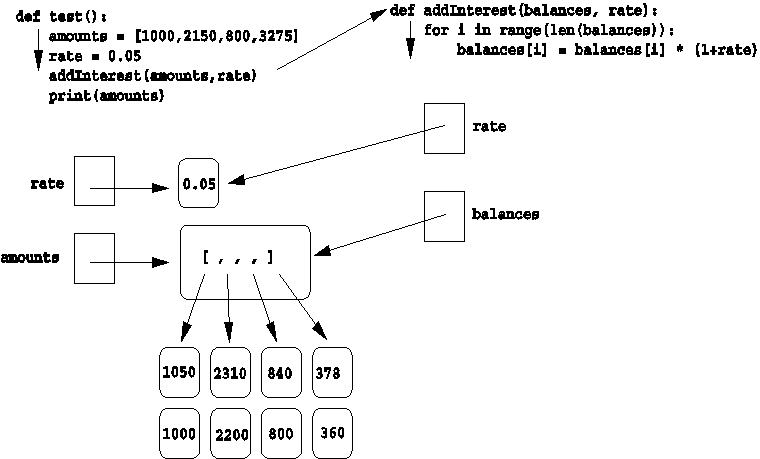
\includegraphics[width=11cm]{pic12}
% \end{center}
\end{frame}

\begin{frame}[fragile,shrink=10]
  \frametitle{Izmena parametara $_{23}$}
\begin{tabular}{p{4cm}p{8cm}}
  \begin{itemize}
    \item[5] stare vrednosti na dijagramu nisu obrisane već su ostavljene da ,,vise`` da bismo naglasili da se nisu promenili brojevi u svojim kutijama, već su novi dodeljeni elementima postojeće liste
    \item[6] stare vrednosti će iz memorije osloboditi \myblue{garbage collection} mehanizam
  \end{itemize}
&
\begin{minted}[linenos=false]{python}
def addInterest(balances, rate):
    for i in range(len(balances)):
        balances[i] = balances[i] *
            (1+rate)

def test():
    amounts = [1000, 2200, 800, 360]
    rate = 0.05
    addInterest(amounts, 0.05)
    print(amounts)
\end{minted}
\end{tabular}
\end{frame}

\begin{frame}[fragile]
  \frametitle{Izmena parametara $_{24}$}
  \begin{itemize}
    \item kada se \texttt{addInterest} završi i kontrola prenese nazad u \texttt{test}
    \item \texttt{amounts} nije promenjen (i dalje je ona stara lista)
    \item ali je stanje te stare liste promenjeno, i to je vidljivo u \texttt{test}-u
  \end{itemize}
\end{frame}

\begin{frame}[fragile]
  \frametitle{Izmena parametara $_{25}$}
  \begin{itemize}
    \item parametri se \myblue{uvek} prenose po vrednosti
    \item ako je vrednost parametra promenljivi objekat, promene na tom objektu će biti vidljive nakon povratka iz funkcije
  \end{itemize}
\end{frame}

\section{*args i **kwargs}

\begin{frame}[fragile]
  \frametitle{Funkcije sa promenljivim brojem parametara}
\begin{minted}[linenos=false]{python}
def my_sum(*args):
    result = 0
    # parametrima pristupamo kao elementima sekvence
    for x in args:
        result += x
    return result

print(my_sum(1, 2, 3))
\end{minted}
  \begin{itemize}
    \item ime \texttt{args} nije obavezno -- može bilo koje drugo
    \item obavezno je navesti \texttt{*} -- \textit{unpacking operator}
  \end{itemize}
\end{frame}

\begin{frame}[fragile]
  \frametitle{Funkcije sa promenljivim brojem parametara}
  \begin{itemize}
    \item \texttt{*args} mora doći posle obaveznih parametara
  \end{itemize}
\begin{minted}[linenos=false]{python}
def print_greeting(greeting, *names):
    for name in names:
        print(greeting + " " + name)

print_greeting("Happy birthday, dear",
               "Joey", "Johnny", "Dee Dee", "Tommy")
\end{minted}
\end{frame}

\begin{frame}[fragile]
  \frametitle{Funkcije sa imenovanim parametrima}
  \begin{itemize}
    \item \texttt{**kwargs} predstavlja imenovane parametre
    \item nepoznate u momentu pisanja funkcije
  \end{itemize}
\begin{minted}[linenos=false]{python}
def concatenate(**kwargs):
    result = ""
    for arg in kwargs:
        result += arg
    result += " "
    for arg in kwargs.values():
        result += arg
    return result

print(concatenate(a="Real", b="Python", c="Is", d="Great", e="!"))
>>> abcde RealPythonIsGreat!
\end{minted}
\end{frame}

\section[Dekoratori]{Dekoratori}

\begin{frame}[fragile]
  \frametitle{Funkcija kao parametar}
  \begin{itemize}
    \item funkcija -- ne poziv funkcije! -- se može proslediti kao parametar
    \item taj parametar se može iskoristiti za poziv dobijene funkcije
    \item ne znamo koja funkcija će biti pozvana u trenutku pisanja tog koda!
  \end{itemize}
\begin{minted}[linenos=false]{python}
def greeter():
    print("Hello")

def repeater(func, times):
    for i in range(times):
        func()

repeater(greeter, 3)
\end{minted}
\end{frame}

\begin{frame}[fragile]
  \frametitle{Funkcija kao parametar}
\begin{minted}[linenos=false]{python}
def greeter():
    print("Hello")

def repeater(func, times):
    for i in range(times):
        func()

repeater(greeter, 3)
\end{minted}
  \begin{itemize}
    \item \texttt{greeter()} je poziv funkcije
    \item \texttt{greeter} je ime funkcije, koje se moze proslediti kao parametar
  \end{itemize}
\end{frame}

\begin{frame}[fragile]
  \frametitle{Funkcija kao parametar}
  \begin{itemize}
    \item primer: \texttt{sort()} ume da sortira, ali će za poređenje elemenata pozivati
    \item \texttt{compare()} koja se može proslediti kao parametar
    \item $\Rightarrow$ možemo da menjamo logiku poređenja, dok algoritam za sortiranje ostaje isti
  \end{itemize}
\end{frame}

\begin{frame}[fragile]
  \frametitle{Funkcija u funkciji}
  \begin{itemize}
    \item funkcija definisana unutar funkcije je vidljiva samo u toj funkciji
  \end{itemize}
\begin{minted}[linenos=false]{python}
def print_integers(values):
    def is_integer(value):
        if type(value) is int:
            return True
        else:
            return False

    for v in values:
        if is_integer(v):
            print(v)


print_integers([1,2,3,"4","tekst", 3.14])
\end{minted}
\end{frame}

\begin{frame}[fragile]
  \frametitle{Obmotavanje funkcije}
  \begin{itemize}
    \item možemo ,,obmotati`` funkciju drugom funkcijom
    \item time dodati ponašanje funkciji nakon što je napisana
  \end{itemize}
\begin{minted}[linenos=false]{python}
def print_call(fn):
    # funkcija prima bilo kakve argumente
    def fn_wrap(*args, **kwargs):
        print("Pozivam %s" % fn.__name__)
        # prosledi bilo kakve argumente funkciji fn
        return fn(*args, **kwargs)

    return fn_wrap  # rezultat funkcije je funkcija!

suma = print_call(sum)  # sum je ugradjena funkcija
print(suma([1, 2, 3, 4]))
\end{minted}
\end{frame}

\begin{frame}[fragile]
  \frametitle{Primer obmotane funkcije}
\begin{minted}[linenos=false]{python}
def print_call(fn):
    def fn_wrap(*args, **kwargs):
        print("Pozivam %s" % fn.__name__)
        retval = fn(*args, **kwargs)
        print("Zavrsen poziv")
        return retval

    return fn_wrap  # rezultat funkcije je funkcija!

def greeter(name):
    return "Hello, %s" % name

greeter = print_call(greeter)  # zadrzavamo staro ime
print(greeter("Branko"))
\end{minted}
\end{frame}

\begin{frame}[fragile]
  \frametitle{Dekorator}
  \begin{itemize}
    \item \myblue{dekorator} je funkcija koja prima funkciju i vraća funkciju
    \item u našem primeru \texttt{print\_call} je dekorator
    \item dodavanje dekoratora na drugu funkciju je lako:
  \end{itemize}
\begin{minted}[linenos=false]{python}
@print_call
def neka_funkcija(a, b, c):
    ...
\end{minted}
  \begin{itemize}
    \item ovo je isto što i
  \end{itemize}
\begin{minted}[linenos=false]{python}
def neka_funkcija(a, b, c):
    ...
neka_funkcija = print_call(neka_funkcija)
\end{minted}
\end{frame}

\section[Closure]{Zatvaranje}

\begin{frame}[fragile,shrink=10]
  \frametitle{Zatvaranje (closure)}
  \begin{itemize}
    \item funkcija ,,vidi`` promenljive iz opsega u kome se nalazi
    \item ali ne može da ih menja
    \end{itemize}
\begin{minted}[linenos=false]{python}
>>> a = 0
>>> def get_a():
...   return a
...
>>> def set_a(val):
...   a = val
...
>>> get_a()
0
>>> a = 3
>>> get_a()
3
>>> set_a(4)
>>> a
3
\end{minted}
\end{frame}

\begin{frame}[fragile]
  \frametitle{Primer zatvaranja}
  \begin{itemize}
    \item funkcija \texttt{nth\_power} je \textit{zatvorena} nad promenljivom \texttt{n}
    \item ima pristup ovoj promenljivoj nakon što izvršavanje programa napusti funkciju \texttt{generate\_power\_func}
    \end{itemize}
\begin{minted}[linenos=false]{python}
def generate_power_func(n):
    def nth_power(x):
        return x**n
    return nth_power

raised_to_4 = generate_power_func(4)
del generate_power_func  # ukloni definiciju ove funkcije
print(raised_to_4(2))

# vrednost n je sacuvana za funkciju raised_to_4
print(raised_to_4.__closure__[0].cell_contents)
\end{minted}
\end{frame}

\section{Strukturiranje programa}

\begin{frame}[fragile]
  \frametitle{Modularni programi}
  \begin{itemize}
    \item do sada smo funkcije koristili kao sredstvo da sprečimo ponavljanje koda
    \item drugi razlog za upotrebu funkcija je pisanje \myblue{modularnih} programa
    \item kako algoritmi koje kreiramo postaju sve složeniji, sve je teže čitati programski kod \\ \ \\
    \item jedan način da se ovo reši je podela algoritma na manje potprograme gde je svaki od njih autonoman (ima smisla sam za sebe)
  \end{itemize}
\end{frame}

\end{document}